\section{Numerical reproducibility and work accounting}
\label{app:reproducibility}
The computational illustrations use the synthetic design in Section~\ref{subsec:cohort-design}. Each scenario has one generated training sample. The training-selection record contains all 144 fold candidates, 48 aggregate positions, and 12 selected full-training models, including numerical eligibility and grid-boundary indicators. The three endpoint corrections in Section~\ref{subsec:polish-results} and the nine fold-level corrections in Section~\ref{subsec:cv-results} are separate sets of Newton calls.

\subsection{Data generation and training folds}
The original synthetic generator uses the Mersenne--Twister, Inversion, and Rejection random-number generator (RNG) settings in R. Matrices are filled by columns, with draw order $\bm{F},\bm{v},\bm{Z},\varepsilon,V$. For scenario index $j$ and replicate $r=1$, the seed rule is $20260929+100000j+100r+\mathrm{role}$, with roles 1 and 2 for training and test samples. The six training samples have event counts 87, 83, 87, 89, 46, and 93 for S1--S6. Population censoring is calibrated by~\eqref{eq:pilot-censoring}; sample censoring retains its generated variation.

The three-fold training-selection analysis uses the event-stratified labels stored with the experiment configuration. Both methods share these labels; each complement contains 80 patients and each validation fold 40. Every mean and PCA transformation is learned on its training complement. The aggregate score retains all within-fold ordered pairs and the common zero-prediction reference in~\eqref{eq:within-fold-cv}.

Earlier evaluations of the generated 400-patient test samples form part of the development record. The cross-validation analysis in this article uses training samples throughout. Assessment of the complete selected procedure on new independent samples is a separate evaluation.

\subsection{Computational work}
A FISTA update is an accepted proximal update, and a Newton update is an accepted active-face correction. The training-selection run has the following work counts; initialization and endpoint verification are counted separately.
\begin{center}
\small
\begin{tabular}{@{}lrrr@{}}
\toprule
Operation & Calls & Accepted updates & Gradient evaluations \\
\midrule
Nuisance initialization & 48 & 3,531 & 3,579 plus 48 full-design \\
FISTA & 156 & 840,530 & 1,680,940 \\
Active-face refinement & 9 & 9 & 18 \\
\bottomrule
\end{tabular}
\end{center}
Endpoint verification additionally uses 165 core and 165 independent pairwise gradient evaluations. The nine refinements require nine Hessian constructions and linear solves; all accept full steps without halving. They occur in UA fold candidates, while the twelve selected full-training refits use no Newton updates. The complete run takes 7,709.2 seconds on the recorded Apple M4 system, including preprocessing, initialization, fitting, verification, and input/output. This is a single-run resource measurement.

\subsection{Source objects and environment}
The reproducibility record retains all aggregate scores, candidate statuses, selected-model summaries, and final coefficient vectors. The identity map specifies the original fields and source hashes. Coefficient nonzero counts use exact comparison with zero. The final standardized objects reconstruct coefficients, the deployment slope, training scores, gradients, and KKT values from the final coefficient vector, including candidates completed by refinement.

The computation uses R 4.5.2 on Apple M4 arm64 with macOS 26.5, Apple Accelerate Basic Linear Algebra Subprograms (BLAS), and Linear Algebra Package (LAPACK) 3.12.1. The original environment includes Python 3.12.15 for independent checks. Package versions and numerical controls are recorded in the accompanying environment and configuration files. Saved R serialized-data (RDS) objects remain the numerical originals; exported tables and figures are linked to those objects. Full trajectories and checkpoints remain in the computational archive. Artwork was generated in R and reformatted by vector-path-preserving operations with PyMuPDF and Ghostscript; plotted coordinates were retained.

Figure~\ref{fig:geometry-updates-supp} presents the accepted-update counterpart of the main-text stationarity trajectories.

\begin{figure}[p]
\centering
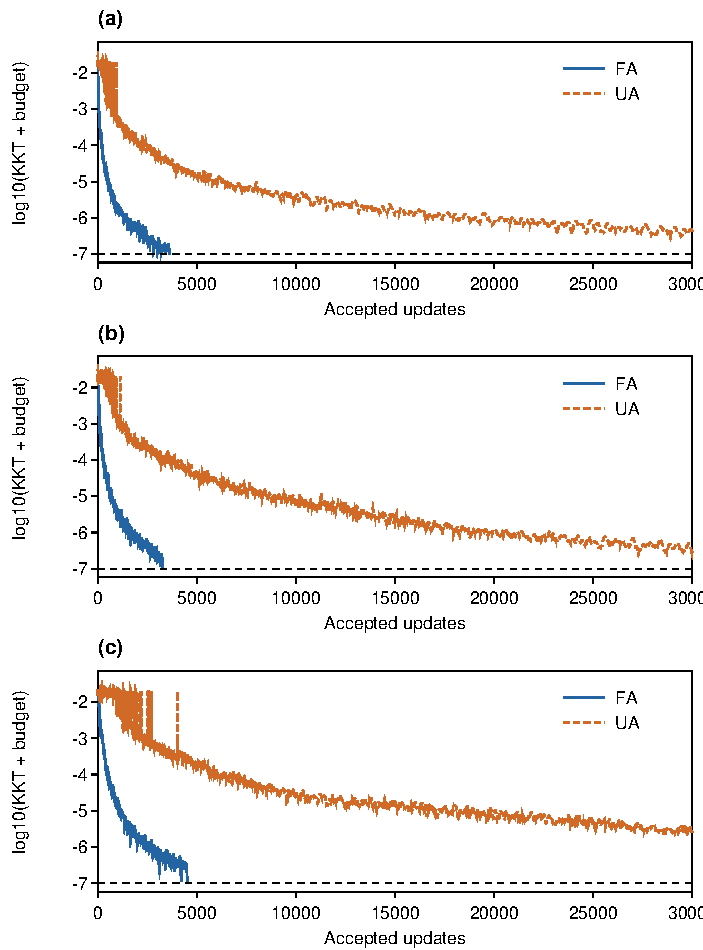
\includegraphics[width=119mm]{figures/FigS1.pdf}
\caption{Full original-coordinate KKT residuals plus tracked numerical budgets versus accepted FISTA updates. The horizontal line is $10^{-7}$. Panels (a), (b), and (c) show S3, S4, and S6. FA is solid and UA is dashed. The fits are the same as Figure~\ref{fig:geometry-gradients}, ending before active-face refinement}
\label{fig:geometry-updates-supp}
\end{figure}

\FloatBarrier
